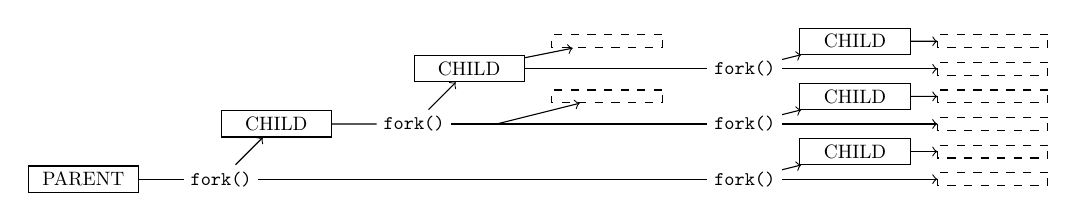
\begin{tikzpicture}[scale=0.7,every node/.style = {scale=0.7}]
\tikzstyle{process} = [minimum width=2cm,draw,];
\tikzstyle{thread} = [minimum width=2cm,draw,dashed]

\node [process] (v1) at (-1.5,0.5) {PARENT};
\node [process] (v2) at (2,1.5) {CHILD};
\node (v3) at (1,0.5) {\texttt{fork()}};

\draw  (v1) edge (v3);
\draw[->]  (v3) edge (v2);
\node (v4) at (4.5,1.5) {\texttt{fork()}};
\draw  (v2) edge (v4);
\node [process] (v5) at (5.5,2.5) {CHILD};
\draw[->]  (v4) edge (v5);
\node [thread] (v9) at (8,2) {};
\node [thread] (v7) at (8,3) {};
\draw[->]  (v5) edge (v7);
\draw[->] (6,1.5) -- (v9);
\node [process] (v11) at (12.5,1) {CHILD};
\node (v10) at (10.5,0.5) {\texttt{fork()}};
\draw  (v3) edge (v10);
\draw [->] (v10) edge (v11);
\node [thread] (v13) at (15,1) {};
\node [thread] (v12) at (15,0.5) {};
\draw[->]  (v10) edge (v12);
\draw[->]  (v11) edge (v13);
\node (v6) at (10.5,1.5) {\texttt{fork()}};
\draw  (v4) edge (v6);
\node (v8) at (10.5,2.5) {\texttt{fork()}};
\draw  (v5) edge (v8);
\node [process] (v15) at (12.5,2) {CHILD};
\node [process] (v14) at (12.5,3) {CHILD};
\draw[->]  (v8) edge (v14);
\draw[->]  (v6) edge (v15);
\node [thread] (v16) at (15,1.5) {};
\node [thread] (v17) at (15,2) {};
\node [thread] (v18) at (15,2.5) {};
\node [thread] (v19) at (15,3) {};
\draw [->]  (v6) edge (v16);
\draw [->]  (v15) edge (v17);
\draw [->] (v8) edge (v18);
\draw [->]  (v14) edge (v19);
\end{tikzpicture}